\documentclass[twoside]{book}

% Packages required by doxygen
\usepackage{fixltx2e}
\usepackage{calc}
\usepackage{doxygen}
\usepackage[export]{adjustbox} % also loads graphicx
\usepackage{graphicx}
\usepackage[utf8]{inputenc}
\usepackage{makeidx}
\usepackage{multicol}
\usepackage{multirow}
\PassOptionsToPackage{warn}{textcomp}
\usepackage{textcomp}
\usepackage[nointegrals]{wasysym}
\usepackage[table]{xcolor}

% Font selection
\usepackage[T1]{fontenc}
\usepackage[scaled=.90]{helvet}
\usepackage{courier}
\usepackage{amssymb}
\usepackage{sectsty}
\renewcommand{\familydefault}{\sfdefault}
\allsectionsfont{%
  \fontseries{bc}\selectfont%
  \color{darkgray}%
}
\renewcommand{\DoxyLabelFont}{%
  \fontseries{bc}\selectfont%
  \color{darkgray}%
}
\newcommand{\+}{\discretionary{\mbox{\scriptsize$\hookleftarrow$}}{}{}}

% Page & text layout
\usepackage{geometry}
\geometry{%
  a4paper,%
  top=2.5cm,%
  bottom=2.5cm,%
  left=2.5cm,%
  right=2.5cm%
}
\tolerance=750
\hfuzz=15pt
\hbadness=750
\setlength{\emergencystretch}{15pt}
\setlength{\parindent}{0cm}
\setlength{\parskip}{0.2cm}
\makeatletter
\renewcommand{\paragraph}{%
  \@startsection{paragraph}{4}{0ex}{-1.0ex}{1.0ex}{%
    \normalfont\normalsize\bfseries\SS@parafont%
  }%
}
\renewcommand{\subparagraph}{%
  \@startsection{subparagraph}{5}{0ex}{-1.0ex}{1.0ex}{%
    \normalfont\normalsize\bfseries\SS@subparafont%
  }%
}
\makeatother

% Headers & footers
\usepackage{fancyhdr}
\pagestyle{fancyplain}
\fancyhead[LE]{\fancyplain{}{\bfseries\thepage}}
\fancyhead[CE]{\fancyplain{}{}}
\fancyhead[RE]{\fancyplain{}{\bfseries\leftmark}}
\fancyhead[LO]{\fancyplain{}{\bfseries\rightmark}}
\fancyhead[CO]{\fancyplain{}{}}
\fancyhead[RO]{\fancyplain{}{\bfseries\thepage}}
\fancyfoot[LE]{\fancyplain{}{}}
\fancyfoot[CE]{\fancyplain{}{}}
\fancyfoot[RE]{\fancyplain{}{\bfseries\scriptsize Generated on Fri Mar 13 2015 03\+:30\+:28 for My Project by Doxygen }}
\fancyfoot[LO]{\fancyplain{}{\bfseries\scriptsize Generated on Fri Mar 13 2015 03\+:30\+:28 for My Project by Doxygen }}
\fancyfoot[CO]{\fancyplain{}{}}
\fancyfoot[RO]{\fancyplain{}{}}
\renewcommand{\footrulewidth}{0.4pt}
\renewcommand{\chaptermark}[1]{%
  \markboth{#1}{}%
}
\renewcommand{\sectionmark}[1]{%
  \markright{\thesection\ #1}%
}

% Indices & bibliography
\usepackage{natbib}
\usepackage[titles]{tocloft}
\setcounter{tocdepth}{3}
\setcounter{secnumdepth}{5}
\makeindex

% Hyperlinks (required, but should be loaded last)
\usepackage{ifpdf}
\ifpdf
  \usepackage[pdftex,pagebackref=true]{hyperref}
\else
  \usepackage[ps2pdf,pagebackref=true]{hyperref}
\fi
\hypersetup{%
  colorlinks=true,%
  linkcolor=blue,%
  citecolor=blue,%
  unicode%
}

% Custom commands
\newcommand{\clearemptydoublepage}{%
  \newpage{\pagestyle{empty}\cleardoublepage}%
}


%===== C O N T E N T S =====

\begin{document}

% Titlepage & ToC
\hypersetup{pageanchor=false,
             bookmarks=true,
             bookmarksnumbered=true,
             pdfencoding=unicode
            }
\pagenumbering{roman}
\begin{titlepage}
\vspace*{7cm}
\begin{center}%
{\Large My Project }\\
\vspace*{1cm}
{\large Generated by Doxygen 1.8.9.1}\\
\vspace*{0.5cm}
{\small Fri Mar 13 2015 03:30:28}\\
\end{center}
\end{titlepage}
\clearemptydoublepage
\tableofcontents
\clearemptydoublepage
\pagenumbering{arabic}
\hypersetup{pageanchor=true}

%--- Begin generated contents ---
\chapter{Hierarchical Index}
\section{Class Hierarchy}
This inheritance list is sorted roughly, but not completely, alphabetically\+:\begin{DoxyCompactList}
\item Q\+Graphics\+Pixmap\+Item\begin{DoxyCompactList}
\item \contentsline{section}{badguy}{\pageref{classbadguy}}{}
\item \contentsline{section}{hostage}{\pageref{classhostage}}{}
\item \contentsline{section}{My\+Player}{\pageref{class_my_player}}{}
\end{DoxyCompactList}
\item Q\+Graphics\+Rect\+Item\begin{DoxyCompactList}
\item \contentsline{section}{Bullet}{\pageref{class_bullet}}{}
\end{DoxyCompactList}
\item Q\+Graphics\+Text\+Item\begin{DoxyCompactList}
\item \contentsline{section}{Score}{\pageref{class_score}}{}
\end{DoxyCompactList}
\item Q\+Graphics\+View\begin{DoxyCompactList}
\item \contentsline{section}{Game}{\pageref{class_game}}{}
\end{DoxyCompactList}
\item Q\+Main\+Window\begin{DoxyCompactList}
\item \contentsline{section}{Main\+Window}{\pageref{class_main_window}}{}
\end{DoxyCompactList}
\item Q\+Object\begin{DoxyCompactList}
\item \contentsline{section}{badguy}{\pageref{classbadguy}}{}
\item \contentsline{section}{Bullet}{\pageref{class_bullet}}{}
\item \contentsline{section}{Endings}{\pageref{class_endings}}{}
\item \contentsline{section}{hostage}{\pageref{classhostage}}{}
\item \contentsline{section}{My\+Player}{\pageref{class_my_player}}{}
\end{DoxyCompactList}
\end{DoxyCompactList}

\chapter{Class Index}
\section{Class List}
Here are the classes, structs, unions and interfaces with brief descriptions\+:\begin{DoxyCompactList}
\item\contentsline{section}{\hyperlink{classbadguy}{badguy} \\*Creates an object for each badguy on the screen }{\pageref{classbadguy}}{}
\item\contentsline{section}{\hyperlink{class_bullet}{Bullet} }{\pageref{class_bullet}}{}
\item\contentsline{section}{\hyperlink{class_endings}{Endings} }{\pageref{class_endings}}{}
\item\contentsline{section}{\hyperlink{class_game}{Game} \\*Inherits from Q\+Graphics view and builds the scene }{\pageref{class_game}}{}
\item\contentsline{section}{\hyperlink{classhostage}{hostage} \\*Creates an object for each hostage on the screen }{\pageref{classhostage}}{}
\item\contentsline{section}{\hyperlink{class_main_window}{Main\+Window} }{\pageref{class_main_window}}{}
\item\contentsline{section}{\hyperlink{class_my_player}{My\+Player} }{\pageref{class_my_player}}{}
\item\contentsline{section}{\hyperlink{class_score}{Score} }{\pageref{class_score}}{}
\end{DoxyCompactList}

\chapter{Class Documentation}
\hypertarget{classbadguy}{}\section{badguy Class Reference}
\label{classbadguy}\index{badguy@{badguy}}


The badguy class creates an object for each badguy on the screen.  




{\ttfamily \#include $<$badguy.\+h$>$}

Inheritance diagram for badguy\+:\begin{figure}[H]
\begin{center}
\leavevmode
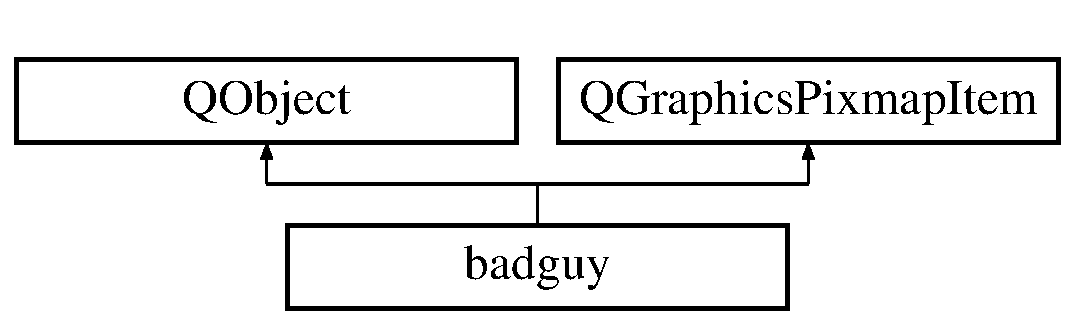
\includegraphics[height=2.000000cm]{classbadguy}
\end{center}
\end{figure}
\subsection*{Public Slots}
\begin{DoxyCompactItemize}
\item 
\hypertarget{classbadguy_afc37049fe30b7644247c05a97cc1d4d9}{}void \hyperlink{classbadguy_afc37049fe30b7644247c05a97cc1d4d9}{move} ()\label{classbadguy_afc37049fe30b7644247c05a97cc1d4d9}

\begin{DoxyCompactList}\small\item\em \hyperlink{classbadguy_afc37049fe30b7644247c05a97cc1d4d9}{badguy\+::move} moves the bad guy left or right within its zone with some randomness \end{DoxyCompactList}\end{DoxyCompactItemize}
\subsection*{Public Member Functions}
\begin{DoxyCompactItemize}
\item 
\hyperlink{classbadguy_a4b6d6fdca626a0267236787fbe20b2ad}{badguy} (\hyperlink{class_game}{Game} $\ast$g)
\begin{DoxyCompactList}\small\item\em \hyperlink{classbadguy_a4b6d6fdca626a0267236787fbe20b2ad}{badguy\+::badguy} \end{DoxyCompactList}\item 
\hypertarget{classbadguy_ad5d09cf91dc849e14f9fe31b3220aaa9}{}\hyperlink{classbadguy_ad5d09cf91dc849e14f9fe31b3220aaa9}{$\sim$badguy} ()\label{classbadguy_ad5d09cf91dc849e14f9fe31b3220aaa9}

\begin{DoxyCompactList}\small\item\em \hyperlink{classbadguy_ad5d09cf91dc849e14f9fe31b3220aaa9}{badguy\+::$\sim$badguy} badguy destructor \end{DoxyCompactList}\end{DoxyCompactItemize}


\subsection{Detailed Description}
The badguy class creates an object for each badguy on the screen. 

\subsection{Constructor \& Destructor Documentation}
\hypertarget{classbadguy_a4b6d6fdca626a0267236787fbe20b2ad}{}\index{badguy@{badguy}!badguy@{badguy}}
\index{badguy@{badguy}!badguy@{badguy}}
\subsubsection[{badguy}]{\setlength{\rightskip}{0pt plus 5cm}badguy\+::badguy (
\begin{DoxyParamCaption}
\item[{{\bf Game} $\ast$}]{g}
\end{DoxyParamCaption}
)}\label{classbadguy_a4b6d6fdca626a0267236787fbe20b2ad}


\hyperlink{classbadguy_a4b6d6fdca626a0267236787fbe20b2ad}{badguy\+::badguy} 


\begin{DoxyParams}{Parameters}
{\em g} & is the parent \hyperlink{class_game}{Game} \\
\hline
\end{DoxyParams}


The documentation for this class was generated from the following files\+:\begin{DoxyCompactItemize}
\item 
badguy.\+h\item 
badguy.\+cpp\end{DoxyCompactItemize}

\hypertarget{class_bullet}{}\section{Bullet Class Reference}
\label{class_bullet}\index{Bullet@{Bullet}}
Inheritance diagram for Bullet\+:\begin{figure}[H]
\begin{center}
\leavevmode
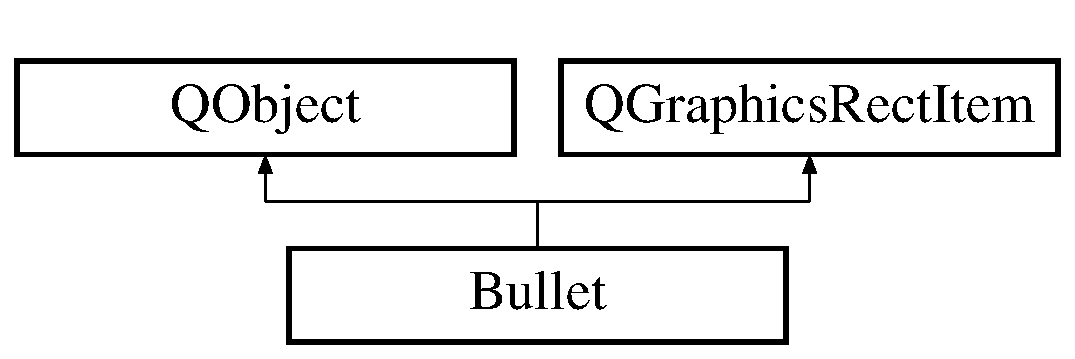
\includegraphics[height=2.000000cm]{class_bullet}
\end{center}
\end{figure}
\subsection*{Public Slots}
\begin{DoxyCompactItemize}
\item 
\hypertarget{class_bullet_a6140db968c42c05e829e142f74f20b16}{}void \hyperlink{class_bullet_a6140db968c42c05e829e142f74f20b16}{move} ()\label{class_bullet_a6140db968c42c05e829e142f74f20b16}

\begin{DoxyCompactList}\small\item\em \hyperlink{class_bullet_a6140db968c42c05e829e142f74f20b16}{Bullet\+::move} moves the bullet and checks to see if anything was hit. \end{DoxyCompactList}\end{DoxyCompactItemize}
\subsection*{Public Member Functions}
\begin{DoxyCompactItemize}
\item 
\hyperlink{class_bullet_a0f8e8b2e3f683cfc930238a7633ce0f2}{Bullet} (\hyperlink{class_my_player}{My\+Player} $\ast$)
\begin{DoxyCompactList}\small\item\em \hyperlink{class_bullet_a0f8e8b2e3f683cfc930238a7633ce0f2}{Bullet\+::\+Bullet}. \end{DoxyCompactList}\item 
\hypertarget{class_bullet_aaeb5cb41d7db89f49007b08b41f1bfcf}{}\hyperlink{class_bullet_aaeb5cb41d7db89f49007b08b41f1bfcf}{$\sim$\+Bullet} ()\label{class_bullet_aaeb5cb41d7db89f49007b08b41f1bfcf}

\begin{DoxyCompactList}\small\item\em \hyperlink{class_bullet_aaeb5cb41d7db89f49007b08b41f1bfcf}{Bullet\+::$\sim$\+Bullet} decrements the bullet count. \end{DoxyCompactList}\end{DoxyCompactItemize}


\subsection{Constructor \& Destructor Documentation}
\hypertarget{class_bullet_a0f8e8b2e3f683cfc930238a7633ce0f2}{}\index{Bullet@{Bullet}!Bullet@{Bullet}}
\index{Bullet@{Bullet}!Bullet@{Bullet}}
\subsubsection[{Bullet}]{\setlength{\rightskip}{0pt plus 5cm}Bullet\+::\+Bullet (
\begin{DoxyParamCaption}
\item[{{\bf My\+Player} $\ast$}]{p}
\end{DoxyParamCaption}
)}\label{class_bullet_a0f8e8b2e3f683cfc930238a7633ce0f2}


\hyperlink{class_bullet_a0f8e8b2e3f683cfc930238a7633ce0f2}{Bullet\+::\+Bullet}. 


\begin{DoxyParams}{Parameters}
{\em p} & points to the player creating the bullet \\
\hline
\end{DoxyParams}


The documentation for this class was generated from the following files\+:\begin{DoxyCompactItemize}
\item 
bullet.\+h\item 
bullet.\+cpp\end{DoxyCompactItemize}

\hypertarget{class_endings}{}\section{Endings Class Reference}
\label{class_endings}\index{Endings@{Endings}}
Inheritance diagram for Endings\+:\begin{figure}[H]
\begin{center}
\leavevmode
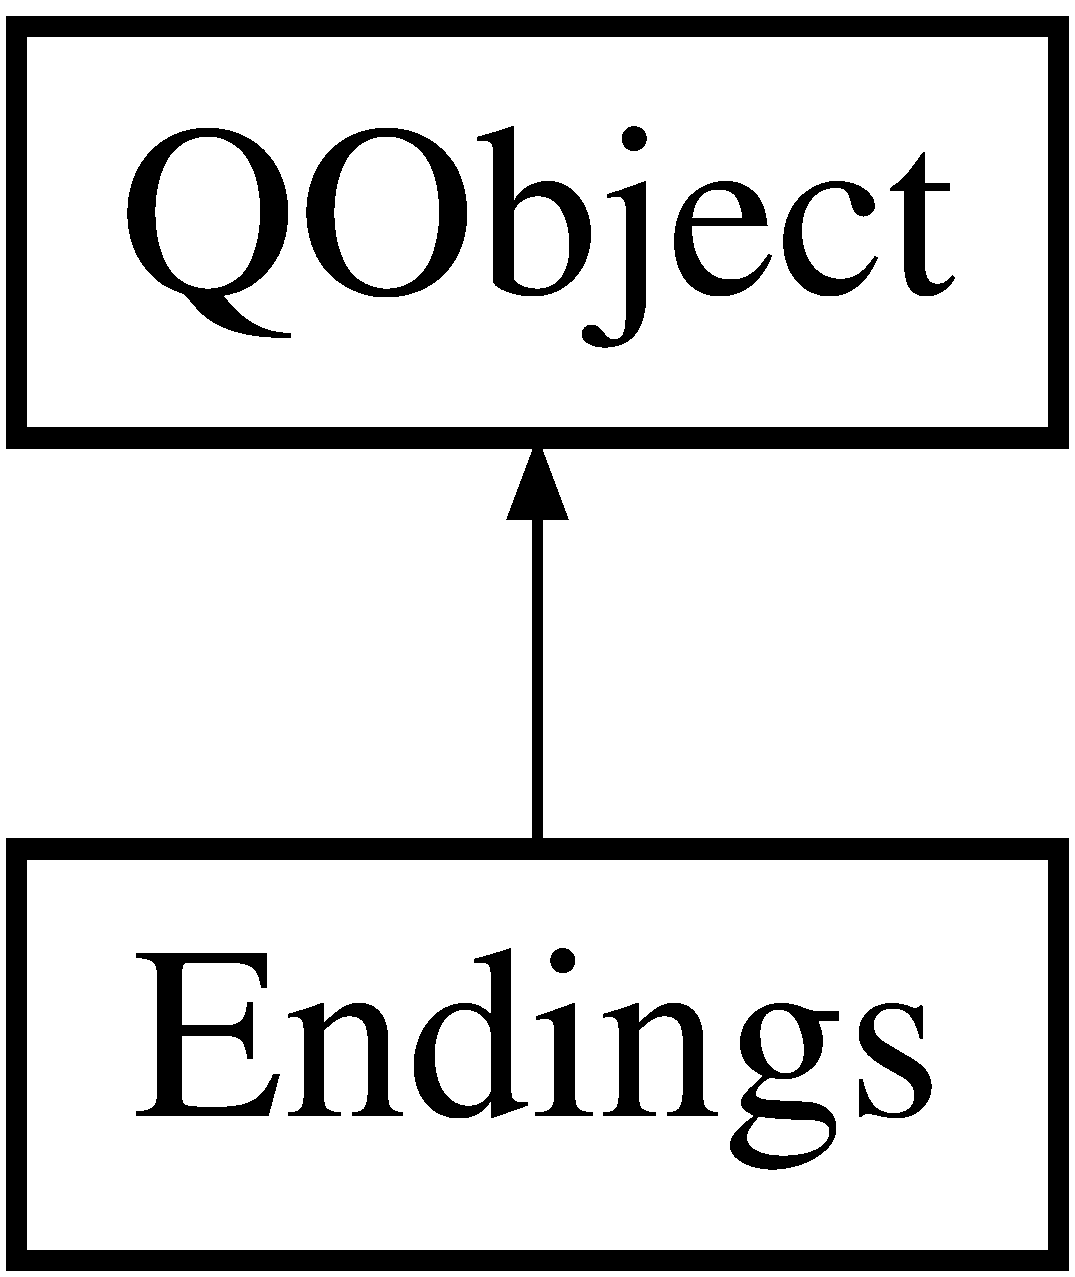
\includegraphics[height=2.000000cm]{class_endings}
\end{center}
\end{figure}
\subsection*{Public Member Functions}
\begin{DoxyCompactItemize}
\item 
\hyperlink{class_endings_aa0a43436cc669e4ddd53260cb04769cf}{Endings} (int type)
\begin{DoxyCompactList}\small\item\em \hyperlink{class_endings_aa0a43436cc669e4ddd53260cb04769cf}{Endings\+::\+Endings}. \end{DoxyCompactList}\end{DoxyCompactItemize}


\subsection{Constructor \& Destructor Documentation}
\hypertarget{class_endings_aa0a43436cc669e4ddd53260cb04769cf}{}\index{Endings@{Endings}!Endings@{Endings}}
\index{Endings@{Endings}!Endings@{Endings}}
\subsubsection[{Endings}]{\setlength{\rightskip}{0pt plus 5cm}Endings\+::\+Endings (
\begin{DoxyParamCaption}
\item[{int}]{type}
\end{DoxyParamCaption}
)}\label{class_endings_aa0a43436cc669e4ddd53260cb04769cf}


\hyperlink{class_endings_aa0a43436cc669e4ddd53260cb04769cf}{Endings\+::\+Endings}. 


\begin{DoxyParams}{Parameters}
{\em type} & is 0 if win, 1 if lose from hostage killed, 2 if lose from player killed \\
\hline
\end{DoxyParams}


The documentation for this class was generated from the following files\+:\begin{DoxyCompactItemize}
\item 
endings.\+h\item 
endings.\+cpp\end{DoxyCompactItemize}

\hypertarget{class_game}{}\section{Game Class Reference}
\label{class_game}\index{Game@{Game}}


The \hyperlink{class_game}{Game} class inherits from Q\+Graphics view and builds the scene.  




{\ttfamily \#include $<$game.\+h$>$}

Inheritance diagram for Game\+:\begin{figure}[H]
\begin{center}
\leavevmode
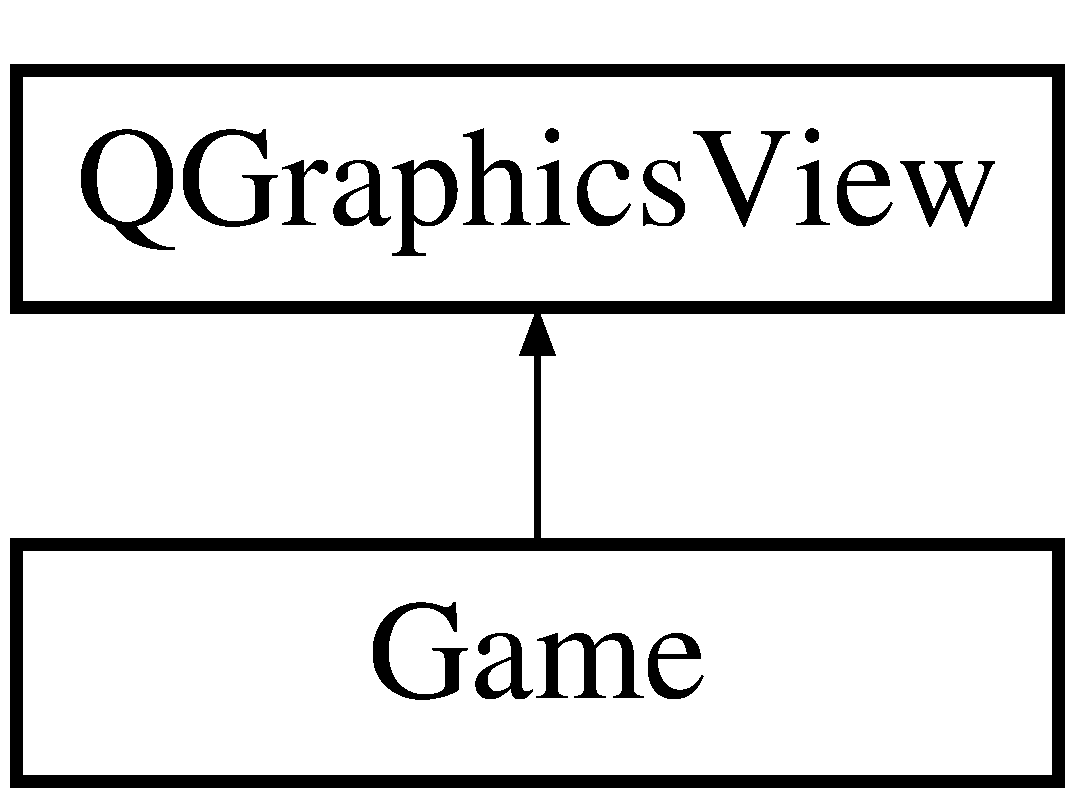
\includegraphics[height=2.000000cm]{class_game}
\end{center}
\end{figure}
\subsection*{Public Slots}
\begin{DoxyCompactItemize}
\item 
\hypertarget{class_game_af3f86c072631ccffc1e3de01bdfd1b88}{}void \hyperlink{class_game_af3f86c072631ccffc1e3de01bdfd1b88}{spawn\+\_\+b} ()\label{class_game_af3f86c072631ccffc1e3de01bdfd1b88}

\begin{DoxyCompactList}\small\item\em spawn\+\_\+b  a new badguy \end{DoxyCompactList}\item 
\hypertarget{class_game_a46fe3c9b6eb40e67d292b71345a5583b}{}void \hyperlink{class_game_a46fe3c9b6eb40e67d292b71345a5583b}{spawn\+\_\+h} ()\label{class_game_a46fe3c9b6eb40e67d292b71345a5583b}

\begin{DoxyCompactList}\small\item\em spawn\+\_\+h  a new hostage \end{DoxyCompactList}\end{DoxyCompactItemize}
\subsection*{Public Member Functions}
\begin{DoxyCompactItemize}
\item 
\hypertarget{class_game_ad59df6562a58a614fda24622d3715b65}{}\hyperlink{class_game_ad59df6562a58a614fda24622d3715b65}{Game} ()\label{class_game_ad59df6562a58a614fda24622d3715b65}

\begin{DoxyCompactList}\small\item\em \hyperlink{class_game_ad59df6562a58a614fda24622d3715b65}{Game\+::\+Game} constructs the \hyperlink{class_game}{Game} scene. \end{DoxyCompactList}\item 
int \hyperlink{class_game_a1723c85835165e0a3353b58350401cd9}{badguys\+\_\+remaining} ()
\begin{DoxyCompactList}\small\item\em badguys\+\_\+remaining \end{DoxyCompactList}\item 
size\+\_\+t \hyperlink{class_game_a6771d472a6adaf1bcc58f997b96f2c16}{badguys\+\_\+onscreen} ()
\begin{DoxyCompactList}\small\item\em badguys\+\_\+onscreen \end{DoxyCompactList}\item 
int \hyperlink{class_game_a6314e99dd420bef0775f61c3d1c30bc7}{max\+\_\+badguys\+\_\+onscreen} ()
\begin{DoxyCompactList}\small\item\em max\+\_\+badguys\+\_\+onscreen \end{DoxyCompactList}\item 
bool \hyperlink{class_game_a978ecd228e6274e192e545b8a49eff9b}{badguy\+\_\+zones} (int n)
\begin{DoxyCompactList}\small\item\em badguy\+\_\+zones \end{DoxyCompactList}\item 
int \hyperlink{class_game_a132981c00605a3a030510aac18e16636}{hostages\+\_\+remaining} ()
\begin{DoxyCompactList}\small\item\em hostages\+\_\+remaining \end{DoxyCompactList}\item 
size\+\_\+t \hyperlink{class_game_a8eb0a78447492976f2af4d69e5f4430e}{hostages\+\_\+onscreen} ()
\begin{DoxyCompactList}\small\item\em hostages\+\_\+onscreen \end{DoxyCompactList}\item 
int \hyperlink{class_game_abceb2d7ac9209b6ff3a2e2b4d727f05d}{max\+\_\+hostages\+\_\+onscreen} ()
\begin{DoxyCompactList}\small\item\em max\+\_\+hostages\+\_\+onscreen \end{DoxyCompactList}\item 
bool \hyperlink{class_game_a90b2ca46a8e37e5a64a9bdce3f4a3e4b}{hostage\+\_\+zones} (int n)
\begin{DoxyCompactList}\small\item\em hostage\+\_\+zones \end{DoxyCompactList}\item 
\hypertarget{class_game_a7406d3975dff0cba5c50115d0f050a45}{}void \hyperlink{class_game_a7406d3975dff0cba5c50115d0f050a45}{badguy\+\_\+killed} ()\label{class_game_a7406d3975dff0cba5c50115d0f050a45}

\begin{DoxyCompactList}\small\item\em badguy\+\_\+killed decrements the number of badguys remaining \end{DoxyCompactList}\item 
void \hyperlink{class_game_ab4807ffbf5ec48e829789fb3390518f1}{set\+\_\+badguys\+\_\+zones} (size\+\_\+t p, bool b)
\begin{DoxyCompactList}\small\item\em set\+\_\+badguys\+\_\+zones \end{DoxyCompactList}\item 
\hypertarget{class_game_a080d1ee7b8efcef5834ffec80e0bbdb1}{}void \hyperlink{class_game_a080d1ee7b8efcef5834ffec80e0bbdb1}{hostage\+\_\+killed} ()\label{class_game_a080d1ee7b8efcef5834ffec80e0bbdb1}

\begin{DoxyCompactList}\small\item\em hostage\+\_\+killed sets flag true when a hostage is killed \end{DoxyCompactList}\item 
void \hyperlink{class_game_ac574b8c3b5287af87d780447c8f34840}{set\+\_\+hostages\+\_\+zones} (size\+\_\+t p, bool b)
\begin{DoxyCompactList}\small\item\em set\+\_\+hostages\+\_\+zones \end{DoxyCompactList}\end{DoxyCompactItemize}
\subsection*{Public Attributes}
\begin{DoxyCompactItemize}
\item 
\hypertarget{class_game_acdf00696bb0d30a7d8472d4bf0cefc1a}{}Q\+Graphics\+Scene $\ast$ {\bfseries scene1}\label{class_game_acdf00696bb0d30a7d8472d4bf0cefc1a}

\item 
\hypertarget{class_game_a1af74ac68938189a26ea16add6edbfaf}{}\hyperlink{class_my_player}{My\+Player} $\ast$ {\bfseries player}\label{class_game_a1af74ac68938189a26ea16add6edbfaf}

\item 
\hypertarget{class_game_ab7a716f587fb6211cd045452b5c9fd02}{}Q\+Graphics\+Text\+Item $\ast$ {\bfseries score}\label{class_game_ab7a716f587fb6211cd045452b5c9fd02}

\end{DoxyCompactItemize}


\subsection{Detailed Description}
The \hyperlink{class_game}{Game} class inherits from Q\+Graphics view and builds the scene. 

\subsection{Member Function Documentation}
\hypertarget{class_game_a978ecd228e6274e192e545b8a49eff9b}{}\index{Game@{Game}!badguy\+\_\+zones@{badguy\+\_\+zones}}
\index{badguy\+\_\+zones@{badguy\+\_\+zones}!Game@{Game}}
\subsubsection[{badguy\+\_\+zones}]{\setlength{\rightskip}{0pt plus 5cm}bool Game\+::badguy\+\_\+zones (
\begin{DoxyParamCaption}
\item[{int}]{n}
\end{DoxyParamCaption}
)\hspace{0.3cm}{\ttfamily [inline]}}\label{class_game_a978ecd228e6274e192e545b8a49eff9b}


badguy\+\_\+zones 


\begin{DoxyParams}{Parameters}
{\em n} & is which zone to check \\
\hline
\end{DoxyParams}
\begin{DoxyReturn}{Returns}
returns true if there is a badguy in the nth zone 
\end{DoxyReturn}
\hypertarget{class_game_a6771d472a6adaf1bcc58f997b96f2c16}{}\index{Game@{Game}!badguys\+\_\+onscreen@{badguys\+\_\+onscreen}}
\index{badguys\+\_\+onscreen@{badguys\+\_\+onscreen}!Game@{Game}}
\subsubsection[{badguys\+\_\+onscreen}]{\setlength{\rightskip}{0pt plus 5cm}size\+\_\+t Game\+::badguys\+\_\+onscreen (
\begin{DoxyParamCaption}
{}
\end{DoxyParamCaption}
)\hspace{0.3cm}{\ttfamily [inline]}}\label{class_game_a6771d472a6adaf1bcc58f997b96f2c16}


badguys\+\_\+onscreen 

\begin{DoxyReturn}{Returns}
the number of badguys currently on the screen 
\end{DoxyReturn}
\hypertarget{class_game_a1723c85835165e0a3353b58350401cd9}{}\index{Game@{Game}!badguys\+\_\+remaining@{badguys\+\_\+remaining}}
\index{badguys\+\_\+remaining@{badguys\+\_\+remaining}!Game@{Game}}
\subsubsection[{badguys\+\_\+remaining}]{\setlength{\rightskip}{0pt plus 5cm}int Game\+::badguys\+\_\+remaining (
\begin{DoxyParamCaption}
{}
\end{DoxyParamCaption}
)\hspace{0.3cm}{\ttfamily [inline]}}\label{class_game_a1723c85835165e0a3353b58350401cd9}


badguys\+\_\+remaining 

\begin{DoxyReturn}{Returns}
the number of badguys remaining 
\end{DoxyReturn}
\hypertarget{class_game_a90b2ca46a8e37e5a64a9bdce3f4a3e4b}{}\index{Game@{Game}!hostage\+\_\+zones@{hostage\+\_\+zones}}
\index{hostage\+\_\+zones@{hostage\+\_\+zones}!Game@{Game}}
\subsubsection[{hostage\+\_\+zones}]{\setlength{\rightskip}{0pt plus 5cm}bool Game\+::hostage\+\_\+zones (
\begin{DoxyParamCaption}
\item[{int}]{n}
\end{DoxyParamCaption}
)\hspace{0.3cm}{\ttfamily [inline]}}\label{class_game_a90b2ca46a8e37e5a64a9bdce3f4a3e4b}


hostage\+\_\+zones 


\begin{DoxyParams}{Parameters}
{\em n} & checks the nth zone \\
\hline
\end{DoxyParams}
\begin{DoxyReturn}{Returns}
true if there is a hostage in the nth zone 
\end{DoxyReturn}
\hypertarget{class_game_a8eb0a78447492976f2af4d69e5f4430e}{}\index{Game@{Game}!hostages\+\_\+onscreen@{hostages\+\_\+onscreen}}
\index{hostages\+\_\+onscreen@{hostages\+\_\+onscreen}!Game@{Game}}
\subsubsection[{hostages\+\_\+onscreen}]{\setlength{\rightskip}{0pt plus 5cm}size\+\_\+t Game\+::hostages\+\_\+onscreen (
\begin{DoxyParamCaption}
{}
\end{DoxyParamCaption}
)\hspace{0.3cm}{\ttfamily [inline]}}\label{class_game_a8eb0a78447492976f2af4d69e5f4430e}


hostages\+\_\+onscreen 

\begin{DoxyReturn}{Returns}
number hostages shown on the screen 
\end{DoxyReturn}
\hypertarget{class_game_a132981c00605a3a030510aac18e16636}{}\index{Game@{Game}!hostages\+\_\+remaining@{hostages\+\_\+remaining}}
\index{hostages\+\_\+remaining@{hostages\+\_\+remaining}!Game@{Game}}
\subsubsection[{hostages\+\_\+remaining}]{\setlength{\rightskip}{0pt plus 5cm}int Game\+::hostages\+\_\+remaining (
\begin{DoxyParamCaption}
{}
\end{DoxyParamCaption}
)\hspace{0.3cm}{\ttfamily [inline]}}\label{class_game_a132981c00605a3a030510aac18e16636}


hostages\+\_\+remaining 

\begin{DoxyReturn}{Returns}
number of hostages remaining 
\end{DoxyReturn}
\hypertarget{class_game_a6314e99dd420bef0775f61c3d1c30bc7}{}\index{Game@{Game}!max\+\_\+badguys\+\_\+onscreen@{max\+\_\+badguys\+\_\+onscreen}}
\index{max\+\_\+badguys\+\_\+onscreen@{max\+\_\+badguys\+\_\+onscreen}!Game@{Game}}
\subsubsection[{max\+\_\+badguys\+\_\+onscreen}]{\setlength{\rightskip}{0pt plus 5cm}int Game\+::max\+\_\+badguys\+\_\+onscreen (
\begin{DoxyParamCaption}
{}
\end{DoxyParamCaption}
)\hspace{0.3cm}{\ttfamily [inline]}}\label{class_game_a6314e99dd420bef0775f61c3d1c30bc7}


max\+\_\+badguys\+\_\+onscreen 

\begin{DoxyReturn}{Returns}
the maximum of badguys to be shown 
\end{DoxyReturn}
\hypertarget{class_game_abceb2d7ac9209b6ff3a2e2b4d727f05d}{}\index{Game@{Game}!max\+\_\+hostages\+\_\+onscreen@{max\+\_\+hostages\+\_\+onscreen}}
\index{max\+\_\+hostages\+\_\+onscreen@{max\+\_\+hostages\+\_\+onscreen}!Game@{Game}}
\subsubsection[{max\+\_\+hostages\+\_\+onscreen}]{\setlength{\rightskip}{0pt plus 5cm}int Game\+::max\+\_\+hostages\+\_\+onscreen (
\begin{DoxyParamCaption}
{}
\end{DoxyParamCaption}
)\hspace{0.3cm}{\ttfamily [inline]}}\label{class_game_abceb2d7ac9209b6ff3a2e2b4d727f05d}


max\+\_\+hostages\+\_\+onscreen 

\begin{DoxyReturn}{Returns}
max number of hostages shown on screen 
\end{DoxyReturn}
\hypertarget{class_game_ab4807ffbf5ec48e829789fb3390518f1}{}\index{Game@{Game}!set\+\_\+badguys\+\_\+zones@{set\+\_\+badguys\+\_\+zones}}
\index{set\+\_\+badguys\+\_\+zones@{set\+\_\+badguys\+\_\+zones}!Game@{Game}}
\subsubsection[{set\+\_\+badguys\+\_\+zones}]{\setlength{\rightskip}{0pt plus 5cm}void Game\+::set\+\_\+badguys\+\_\+zones (
\begin{DoxyParamCaption}
\item[{size\+\_\+t}]{p, }
\item[{bool}]{b}
\end{DoxyParamCaption}
)\hspace{0.3cm}{\ttfamily [inline]}}\label{class_game_ab4807ffbf5ec48e829789fb3390518f1}


set\+\_\+badguys\+\_\+zones 


\begin{DoxyParams}{Parameters}
{\em p} & is the pth zone \\
\hline
{\em b} & is true or false sets true or false when a a badguy is added to or removed from a zone \\
\hline
\end{DoxyParams}
\hypertarget{class_game_ac574b8c3b5287af87d780447c8f34840}{}\index{Game@{Game}!set\+\_\+hostages\+\_\+zones@{set\+\_\+hostages\+\_\+zones}}
\index{set\+\_\+hostages\+\_\+zones@{set\+\_\+hostages\+\_\+zones}!Game@{Game}}
\subsubsection[{set\+\_\+hostages\+\_\+zones}]{\setlength{\rightskip}{0pt plus 5cm}void Game\+::set\+\_\+hostages\+\_\+zones (
\begin{DoxyParamCaption}
\item[{size\+\_\+t}]{p, }
\item[{bool}]{b}
\end{DoxyParamCaption}
)\hspace{0.3cm}{\ttfamily [inline]}}\label{class_game_ac574b8c3b5287af87d780447c8f34840}


set\+\_\+hostages\+\_\+zones 


\begin{DoxyParams}{Parameters}
{\em p} & is the pth zone \\
\hline
{\em b} & is true or false sets true or false when a a hostage is added to or removed from a zone \\
\hline
\end{DoxyParams}


The documentation for this class was generated from the following files\+:\begin{DoxyCompactItemize}
\item 
game.\+h\item 
game.\+cpp\end{DoxyCompactItemize}

\hypertarget{classhostage}{}\section{hostage Class Reference}
\label{classhostage}\index{hostage@{hostage}}


The hostage class creates an object for each hostage on the screen.  




{\ttfamily \#include $<$hostage.\+h$>$}

Inheritance diagram for hostage\+:\begin{figure}[H]
\begin{center}
\leavevmode
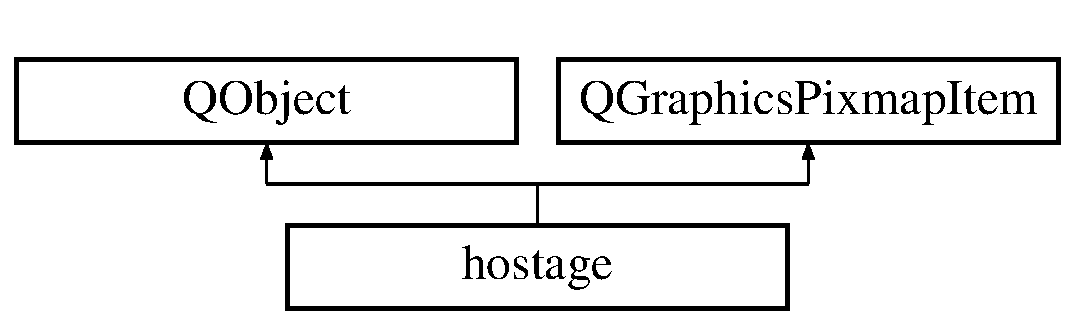
\includegraphics[height=2.000000cm]{classhostage}
\end{center}
\end{figure}
\subsection*{Public Slots}
\begin{DoxyCompactItemize}
\item 
\hypertarget{classhostage_a5f63e03a71d6cee9c7253efd6614d66a}{}void \hyperlink{classhostage_a5f63e03a71d6cee9c7253efd6614d66a}{move} ()\label{classhostage_a5f63e03a71d6cee9c7253efd6614d66a}

\begin{DoxyCompactList}\small\item\em \hyperlink{classhostage_a5f63e03a71d6cee9c7253efd6614d66a}{hostage\+::move} moves the hostage left or right within its zone \end{DoxyCompactList}\end{DoxyCompactItemize}
\subsection*{Public Member Functions}
\begin{DoxyCompactItemize}
\item 
\hyperlink{classhostage_a289f13eb03abb9eb0d683d51faf292fc}{hostage} (\hyperlink{class_game}{Game} $\ast$g)
\begin{DoxyCompactList}\small\item\em \hyperlink{classhostage_a289f13eb03abb9eb0d683d51faf292fc}{hostage\+::hostage} \end{DoxyCompactList}\end{DoxyCompactItemize}


\subsection{Detailed Description}
The hostage class creates an object for each hostage on the screen. 

\subsection{Constructor \& Destructor Documentation}
\hypertarget{classhostage_a289f13eb03abb9eb0d683d51faf292fc}{}\index{hostage@{hostage}!hostage@{hostage}}
\index{hostage@{hostage}!hostage@{hostage}}
\subsubsection[{hostage}]{\setlength{\rightskip}{0pt plus 5cm}hostage\+::hostage (
\begin{DoxyParamCaption}
\item[{{\bf Game} $\ast$}]{g}
\end{DoxyParamCaption}
)}\label{classhostage_a289f13eb03abb9eb0d683d51faf292fc}


\hyperlink{classhostage_a289f13eb03abb9eb0d683d51faf292fc}{hostage\+::hostage} 


\begin{DoxyParams}{Parameters}
{\em g} & is the parent \hyperlink{class_game}{Game} \\
\hline
\end{DoxyParams}


The documentation for this class was generated from the following files\+:\begin{DoxyCompactItemize}
\item 
hostage.\+h\item 
hostage.\+cpp\end{DoxyCompactItemize}

\hypertarget{class_main_window}{}\section{Main\+Window Class Reference}
\label{class_main_window}\index{Main\+Window@{Main\+Window}}
Inheritance diagram for Main\+Window\+:\begin{figure}[H]
\begin{center}
\leavevmode
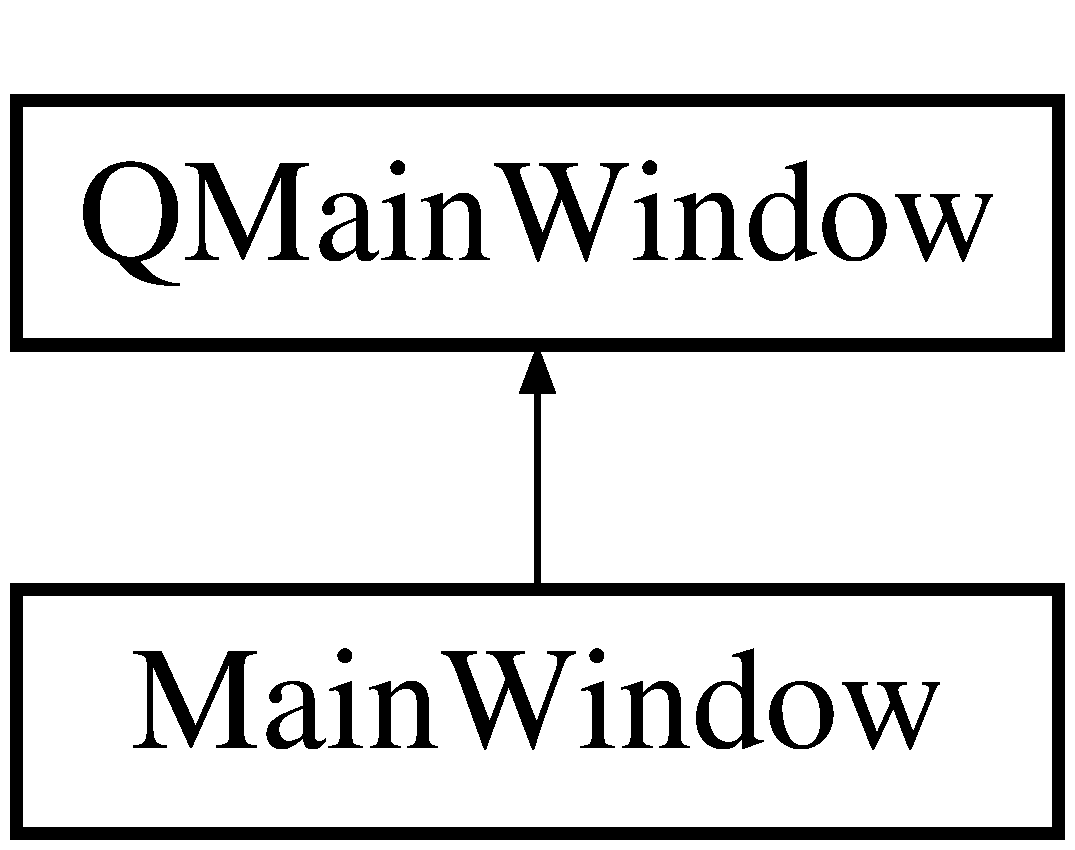
\includegraphics[height=2.000000cm]{class_main_window}
\end{center}
\end{figure}
\subsection*{Public Member Functions}
\begin{DoxyCompactItemize}
\item 
\hyperlink{class_main_window_a8b244be8b7b7db1b08de2a2acb9409db}{Main\+Window} (Q\+Widget $\ast$parent=0)
\begin{DoxyCompactList}\small\item\em \hyperlink{class_main_window_a8b244be8b7b7db1b08de2a2acb9409db}{Main\+Window\+::\+Main\+Window}. \end{DoxyCompactList}\item 
void \hyperlink{class_main_window_a8716d52cdf2b17540512951c2db27675}{set\+Game} (\hyperlink{class_game}{Game} $\ast$g)
\begin{DoxyCompactList}\small\item\em \hyperlink{class_main_window_a8716d52cdf2b17540512951c2db27675}{Main\+Window\+::set\+Game}. \end{DoxyCompactList}\end{DoxyCompactItemize}


\subsection{Constructor \& Destructor Documentation}
\hypertarget{class_main_window_a8b244be8b7b7db1b08de2a2acb9409db}{}\index{Main\+Window@{Main\+Window}!Main\+Window@{Main\+Window}}
\index{Main\+Window@{Main\+Window}!Main\+Window@{Main\+Window}}
\subsubsection[{Main\+Window}]{\setlength{\rightskip}{0pt plus 5cm}Main\+Window\+::\+Main\+Window (
\begin{DoxyParamCaption}
\item[{Q\+Widget $\ast$}]{parent = {\ttfamily 0}}
\end{DoxyParamCaption}
)\hspace{0.3cm}{\ttfamily [explicit]}}\label{class_main_window_a8b244be8b7b7db1b08de2a2acb9409db}


\hyperlink{class_main_window_a8b244be8b7b7db1b08de2a2acb9409db}{Main\+Window\+::\+Main\+Window}. 


\begin{DoxyParams}{Parameters}
{\em parent} & is the parent widget constructs the intro message window \\
\hline
\end{DoxyParams}


\subsection{Member Function Documentation}
\hypertarget{class_main_window_a8716d52cdf2b17540512951c2db27675}{}\index{Main\+Window@{Main\+Window}!set\+Game@{set\+Game}}
\index{set\+Game@{set\+Game}!Main\+Window@{Main\+Window}}
\subsubsection[{set\+Game}]{\setlength{\rightskip}{0pt plus 5cm}void Main\+Window\+::set\+Game (
\begin{DoxyParamCaption}
\item[{{\bf Game} $\ast$}]{g}
\end{DoxyParamCaption}
)}\label{class_main_window_a8716d52cdf2b17540512951c2db27675}


\hyperlink{class_main_window_a8716d52cdf2b17540512951c2db27675}{Main\+Window\+::set\+Game}. 


\begin{DoxyParams}{Parameters}
{\em g} & points to a \hyperlink{class_game}{Game} object opens the game when the start button is clicked \\
\hline
\end{DoxyParams}


The documentation for this class was generated from the following files\+:\begin{DoxyCompactItemize}
\item 
mainwindow.\+h\item 
mainwindow.\+cpp\end{DoxyCompactItemize}

\hypertarget{class_my_player}{}\section{My\+Player Class Reference}
\label{class_my_player}\index{My\+Player@{My\+Player}}
Inheritance diagram for My\+Player\+:\begin{figure}[H]
\begin{center}
\leavevmode
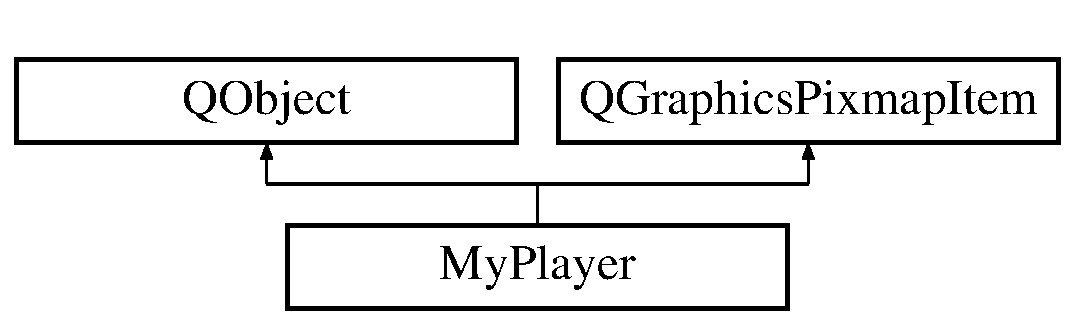
\includegraphics[height=2.000000cm]{class_my_player}
\end{center}
\end{figure}
\subsection*{Public Slots}
\begin{DoxyCompactItemize}
\item 
\hypertarget{class_my_player_a285f57dbb01b962385de6f323f1c847c}{}void \hyperlink{class_my_player_a285f57dbb01b962385de6f323f1c847c}{move} ()\label{class_my_player_a285f57dbb01b962385de6f323f1c847c}

\begin{DoxyCompactList}\small\item\em \hyperlink{class_my_player_a285f57dbb01b962385de6f323f1c847c}{My\+Player\+::move} moves the player. \end{DoxyCompactList}\item 
\hypertarget{class_my_player_ac00726202004d1d5aef9b7410bfce6ad}{}void \hyperlink{class_my_player_ac00726202004d1d5aef9b7410bfce6ad}{shoot} ()\label{class_my_player_ac00726202004d1d5aef9b7410bfce6ad}

\begin{DoxyCompactList}\small\item\em \hyperlink{class_my_player_ac00726202004d1d5aef9b7410bfce6ad}{My\+Player\+::shoot} shoot bullets. \end{DoxyCompactList}\end{DoxyCompactItemize}
\subsection*{Public Member Functions}
\begin{DoxyCompactItemize}
\item 
\hyperlink{class_my_player_a43316e7e70cd8f196f6031f987068d20}{My\+Player} (\hyperlink{class_game}{Game} $\ast$g)
\begin{DoxyCompactList}\small\item\em \hyperlink{class_my_player_a43316e7e70cd8f196f6031f987068d20}{My\+Player\+::\+My\+Player}. \end{DoxyCompactList}\item 
void \hyperlink{class_my_player_aba7afb69ba4dc7679c91bc204f8a5543}{key\+Press\+Event} (Q\+Key\+Event $\ast$)
\begin{DoxyCompactList}\small\item\em \hyperlink{class_my_player_aba7afb69ba4dc7679c91bc204f8a5543}{My\+Player\+::key\+Press\+Event}. \end{DoxyCompactList}\item 
void \hyperlink{class_my_player_a72361f5f9b601a37e3cda0207657d2e9}{key\+Release\+Event} (Q\+Key\+Event $\ast$)
\begin{DoxyCompactList}\small\item\em \hyperlink{class_my_player_a72361f5f9b601a37e3cda0207657d2e9}{My\+Player\+::key\+Release\+Event}. \end{DoxyCompactList}\end{DoxyCompactItemize}
\subsection*{Friends}
\begin{DoxyCompactItemize}
\item 
\hypertarget{class_my_player_a24819047809c73786cf241ae7546a7cd}{}class {\bfseries Bullet}\label{class_my_player_a24819047809c73786cf241ae7546a7cd}

\end{DoxyCompactItemize}


\subsection{Constructor \& Destructor Documentation}
\hypertarget{class_my_player_a43316e7e70cd8f196f6031f987068d20}{}\index{My\+Player@{My\+Player}!My\+Player@{My\+Player}}
\index{My\+Player@{My\+Player}!My\+Player@{My\+Player}}
\subsubsection[{My\+Player}]{\setlength{\rightskip}{0pt plus 5cm}My\+Player\+::\+My\+Player (
\begin{DoxyParamCaption}
\item[{{\bf Game} $\ast$}]{g}
\end{DoxyParamCaption}
)}\label{class_my_player_a43316e7e70cd8f196f6031f987068d20}


\hyperlink{class_my_player_a43316e7e70cd8f196f6031f987068d20}{My\+Player\+::\+My\+Player}. 


\begin{DoxyParams}{Parameters}
{\em g} & points to the parent \hyperlink{class_game}{Game} \\
\hline
\end{DoxyParams}


\subsection{Member Function Documentation}
\hypertarget{class_my_player_aba7afb69ba4dc7679c91bc204f8a5543}{}\index{My\+Player@{My\+Player}!key\+Press\+Event@{key\+Press\+Event}}
\index{key\+Press\+Event@{key\+Press\+Event}!My\+Player@{My\+Player}}
\subsubsection[{key\+Press\+Event}]{\setlength{\rightskip}{0pt plus 5cm}void My\+Player\+::key\+Press\+Event (
\begin{DoxyParamCaption}
\item[{Q\+Key\+Event $\ast$}]{event}
\end{DoxyParamCaption}
)}\label{class_my_player_aba7afb69ba4dc7679c91bc204f8a5543}


\hyperlink{class_my_player_aba7afb69ba4dc7679c91bc204f8a5543}{My\+Player\+::key\+Press\+Event}. 


\begin{DoxyParams}{Parameters}
{\em event} & is a key press event adds pressed keys to the keys vecctor \\
\hline
\end{DoxyParams}
\hypertarget{class_my_player_a72361f5f9b601a37e3cda0207657d2e9}{}\index{My\+Player@{My\+Player}!key\+Release\+Event@{key\+Release\+Event}}
\index{key\+Release\+Event@{key\+Release\+Event}!My\+Player@{My\+Player}}
\subsubsection[{key\+Release\+Event}]{\setlength{\rightskip}{0pt plus 5cm}void My\+Player\+::key\+Release\+Event (
\begin{DoxyParamCaption}
\item[{Q\+Key\+Event $\ast$}]{event}
\end{DoxyParamCaption}
)}\label{class_my_player_a72361f5f9b601a37e3cda0207657d2e9}


\hyperlink{class_my_player_a72361f5f9b601a37e3cda0207657d2e9}{My\+Player\+::key\+Release\+Event}. 


\begin{DoxyParams}{Parameters}
{\em event} & is a key\+Release\+Event removes released keys from the keys vector \\
\hline
\end{DoxyParams}


The documentation for this class was generated from the following files\+:\begin{DoxyCompactItemize}
\item 
myplayer.\+h\item 
myplayer.\+cpp\end{DoxyCompactItemize}

\hypertarget{class_score}{}\section{Score Class Reference}
\label{class_score}\index{Score@{Score}}
Inheritance diagram for Score\+:\begin{figure}[H]
\begin{center}
\leavevmode
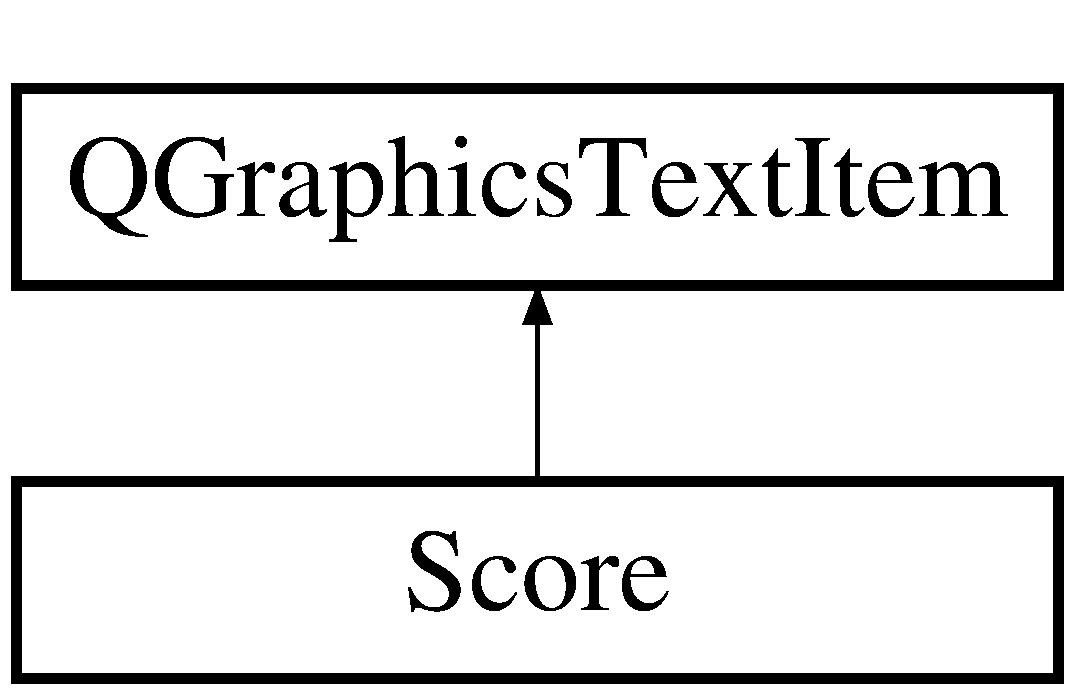
\includegraphics[height=2.000000cm]{class_score}
\end{center}
\end{figure}
\subsection*{Public Member Functions}
\begin{DoxyCompactItemize}
\item 
\hypertarget{class_score_ad50f4da3306f8f920c23b33badae9d2d}{}{\bfseries Score} (\hyperlink{class_game}{Game} $\ast$g)\label{class_score_ad50f4da3306f8f920c23b33badae9d2d}

\end{DoxyCompactItemize}


The documentation for this class was generated from the following files\+:\begin{DoxyCompactItemize}
\item 
score.\+h\item 
score.\+cpp\end{DoxyCompactItemize}

%--- End generated contents ---

% Index
\backmatter
\newpage
\phantomsection
\clearemptydoublepage
\addcontentsline{toc}{chapter}{Index}
\printindex

\end{document}
